\chapter{Resultados}
\label{champ:results}
\bigskip
\barra
\bigskip

\textbf{Nota: Este apartado esta siendo traducido del artículo que se presentara en el workshop PDSEC 2014 en el Conrgeso IEEE IPDPS 2014, adicionalmente se complementara con resultados de pruebas en progreso}.\\

El algoritmo propuesto en la Capítulo \ref{champ:PBSGR} fue implementando utilizando OpenMP. Las pruebas fueron realizadas en una computadora con un procesador Intel(R) Core(TM) i7 CPU  Extreme Edition a una velocidad de 3.47GHz y con 16GB de RAM. La versión secuencial descrita en el Capítulo \ref{champ:BSGR} se ejecuto en un solo procesador.\\

Nuestra solución básica secuencial (llamada en este capítulo como BSGR: Solución Básica considerando $GR$), con la cual se pueden generar redes porosas que cumplen con el $PC$ y las $RG$; sin embargo, el ordenamiento de los enlaces y la búsqueda de configuraciones válidas esto se trasforma en que se requiere un mayor número de cálculos que la versión secuencial NoMISS como se muestra ne la Figura \ref{fig:timevartraslape}. Podemos observar en esta figura  con $L=100$ que con BSGR y su versión paralela solo se podrán construir redes porosas con traslapes bajos, en comparación con la versión secuencial de NoMISS, con la cual en las referencias \cite{ref4} y \cite{ref3} donde se alcanzaron altos traslapes.\\

Comparamos la versión paralela de BSGR en las redes porosas con bajo diferentes valores de $\Omega$. En la Figura \ref{fig:timevartraslape} podemos observar que la versión BSGR Paralela (utilizando 8 hilos) supera a la versión BSGR independientemente de los valores del traslape.\\

Es evidente que el valor del traslape $\Omega$ alcanzado en las redes que consideran el cumplimiento del $PC$ y las $RG$, es relativamente bajo ($\Omega<1$). Este hecho se debe a la restricción impuesta por las restricciones geométricas. Esto último se ilustra en las ecuaciones \ref{eq:eq02} y \ref{eq:eq03}:

\begin{equation}
B_C(R_S) \geq S(R_S)
\label{eq:eq02}
\end{equation}

\begin{eqnarray}
\nonumber \\
B_C(R_S) = & \{\int\limits^{R_S} ... \int\limits_{0} F_B(R_{B1})\; ... \; F_B(R_{BC})dR_{B1} \nonumber \\
& \; \ldots \; dR_{BC} \}^{1/C}
\label{eq:eq03}
\end{eqnarray}

donde $B_C(R_S)$ es corresponde el volumen definido por la ecuación \ref{eq:eq03}; esta se relaciona con el conjunto de enlaces que pueden ser conectados a un sitio, evitando al mismo tiempo la existencia de interferencias entre ellos. $S(R_S)$ es la fracción de sitios que son de tamaño $R_S$ o más pequeños.\\

Las ecuaciones \ref{eq:eq02} y \ref{eq:eq03} restringen el valor de traslape como se muestra en \cite{ref5}, ya que la definición matemática de $B_C(R_S)$ impide en si alcanzar valores cercanos a la unidad, es por eso que se obtienen valores de traslape son $\Omega<1$.\\

\begin{figure}[hbtp]
\centering
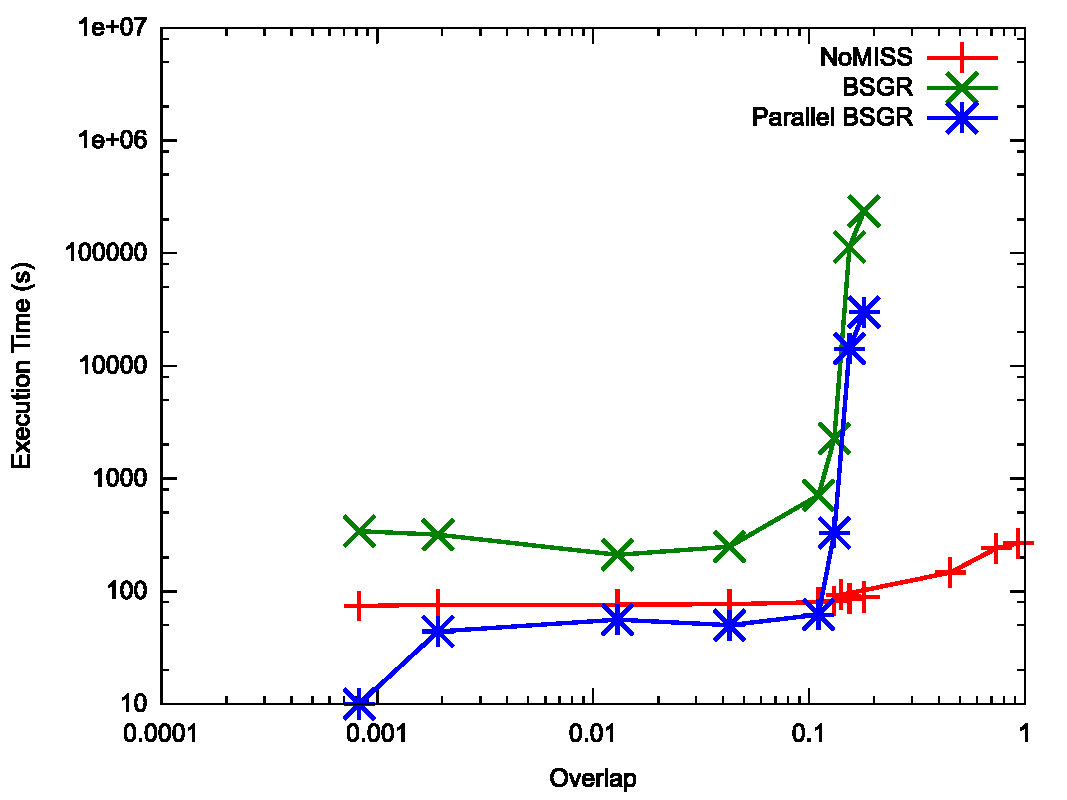
\includegraphics[width=4in]{img/variatraslape.pdf}
\caption{Tiempos de ejecución de NoMISS, BSGR y BSGR paralelo, bajo diferentes valores de $\Omega$ (escala logarítmica)}
\label{fig:timevartraslape}
\end{figure}

La Figura \ref{fig:timenuevo} muestra el tiepo de ejecución requerido para crear una red porosa con $L=100$, $\Omega=0.15$, $ClusterSize=32$, y $NClusters=30$ utilizando un número de hilos diferente. El tiempo de ejecución en paralelo en general disminuye mientras aumenta el número de hilos. Podemos observar en algunos casos, como cuando el número e hilos  es igual a 6 y 14, el tiempo de ejecución no disminuye; creemos que estos casos se deben a la siembra aleatoria de clusters lo cual genera un número mayor de violaciones a las $RG$ que en los otros casos, al tener un mayor número de violaciones el tiempo que lleva generar una red porosa válida es mayor.\\
 
\begin{figure}[hbtp]
\centering
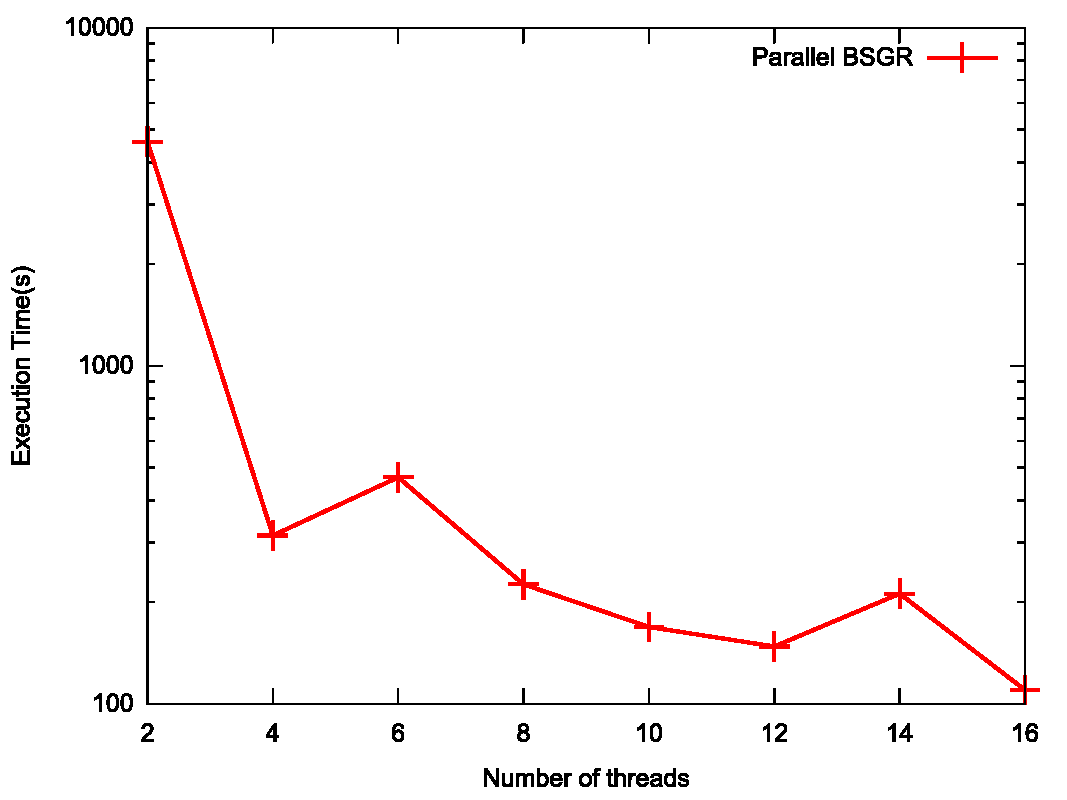
\includegraphics[width=4in]{img/tiempoPar2To16.pdf}
\caption{Tiempos de ejecución de BSGR Paralelo utilizando de 2 a 16 hilos (escala logarítmica)}
\label{fig:timenuevo}
\end{figure}

En la Figura \ref{fig:redes} observamos un ejemplo gráfico de una red porosa con $L=100$ y $\Omega=0.15$, obteniendo a partir de la versión BSGR (Figura \ref{fig:red1}), así como de la versión BSGR Paralela (Figura \ref{fig:red2}) utilizando 8 hilos. Estas imágenes representas redes porosas después del sembrado de cluster de poros y los pasos de asignación de enlaces; es decir, que se permite la existencia de violaciones a las $RG$. El código de color asignado en las Figuras \ref{fig:redes}, \ref{fig:redes2} y \ref{fig:redes3} es como sigue: los poros grandes se muestran de color rojo, los poros de tamaño medio de color azul y los poros pequeños en color azul claro.\\

La Figura \ref{fig:redes2} muestra las anteriores redes porosas después de eliminar por completo las violaciones a las $RG$ a través de la aplicación de $MCs$. En las Figuras \ref{fig:red3} y \ref{fig:red4}, se puede observar que aun quedan estructuras de poro cúbicas que en redes porosas reales no se presentan.\\

Después de aplicar un número adicional de $MCs$ le ísotropia de la red se mejora, obteniendo redes porosas que representan redes porosas más reales, como se muestra en las Figuras \ref{fig:red5} y \ref{fig:red6}.\\

\begin{figure}[hbtp]
\centering
\begin{tabular}{cc}
\subfloat[$ $]{
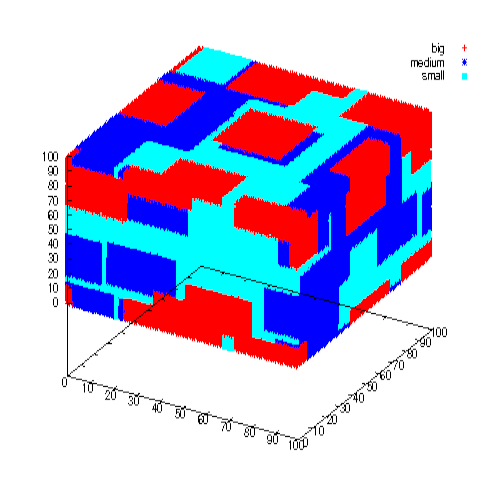
\includegraphics[width=2.3in]{img/redsec100.png}
\label{fig:red1}}
& \subfloat[$ $]{
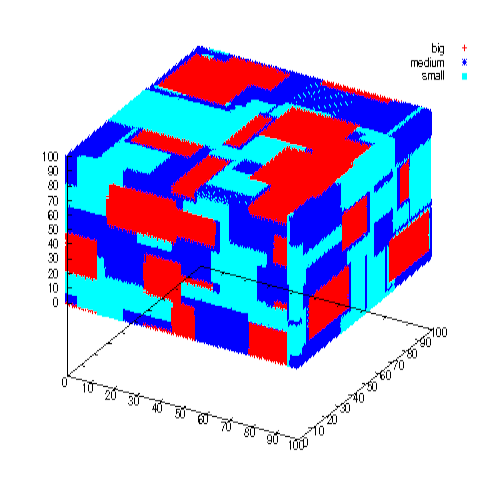
\includegraphics[width=2.3in]{img/redpar100.png}
\label{fig:red2}}
\end{tabular}
\caption{Redes porosas que permiten violaciones a las $GR$, con $L=100$ y $\Omega=0.15$, obtenidas con (a) BSGR y (b) BSGR Paralelo utilizando 8 hilos}
\label{fig:redes}
\end{figure}

\begin{figure}[hbtp]
\centering
\begin{tabular}{cc}
\subfloat[$ $]{
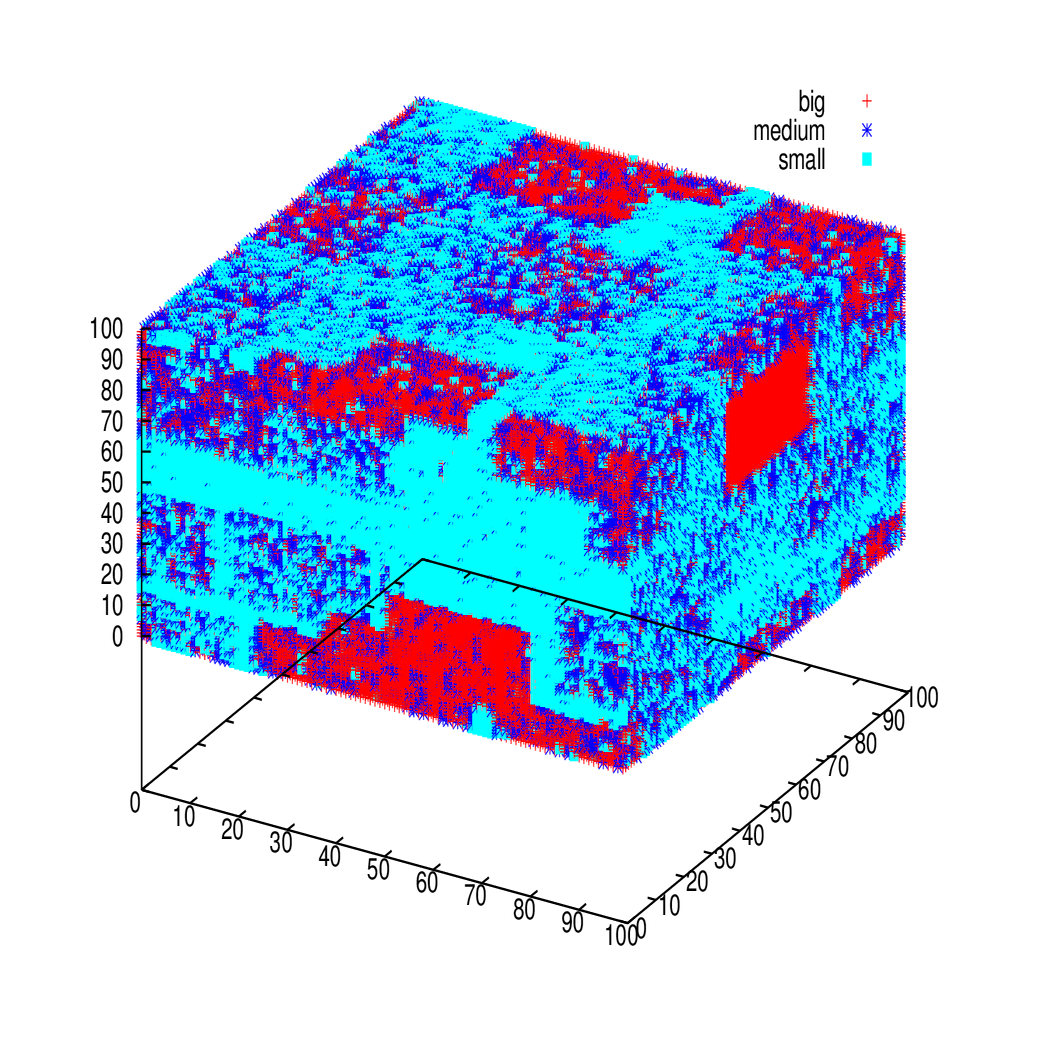
\includegraphics[width=2.3in]{img/red3.png}
\label{fig:red3}}
& \subfloat[$ $]{
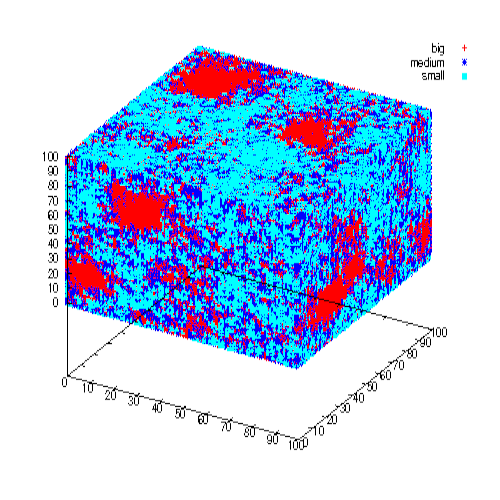
\includegraphics[width=2.3in]{img/red4.png}
\label{fig:red4}}
\end{tabular}
\caption{Redes porosas libre de violaciones a las $GR$, con $L=100$ y $\Omega=0.15$, obtenidas con (a) BSGR  and (b) BSGR Paralelo utilizando 8 hilos}
\label{fig:redes2}
\end{figure}

%\begin{figure}[h]
%\centering
%\begin{tabular}{cc}
%\subfloat[$ $]{
%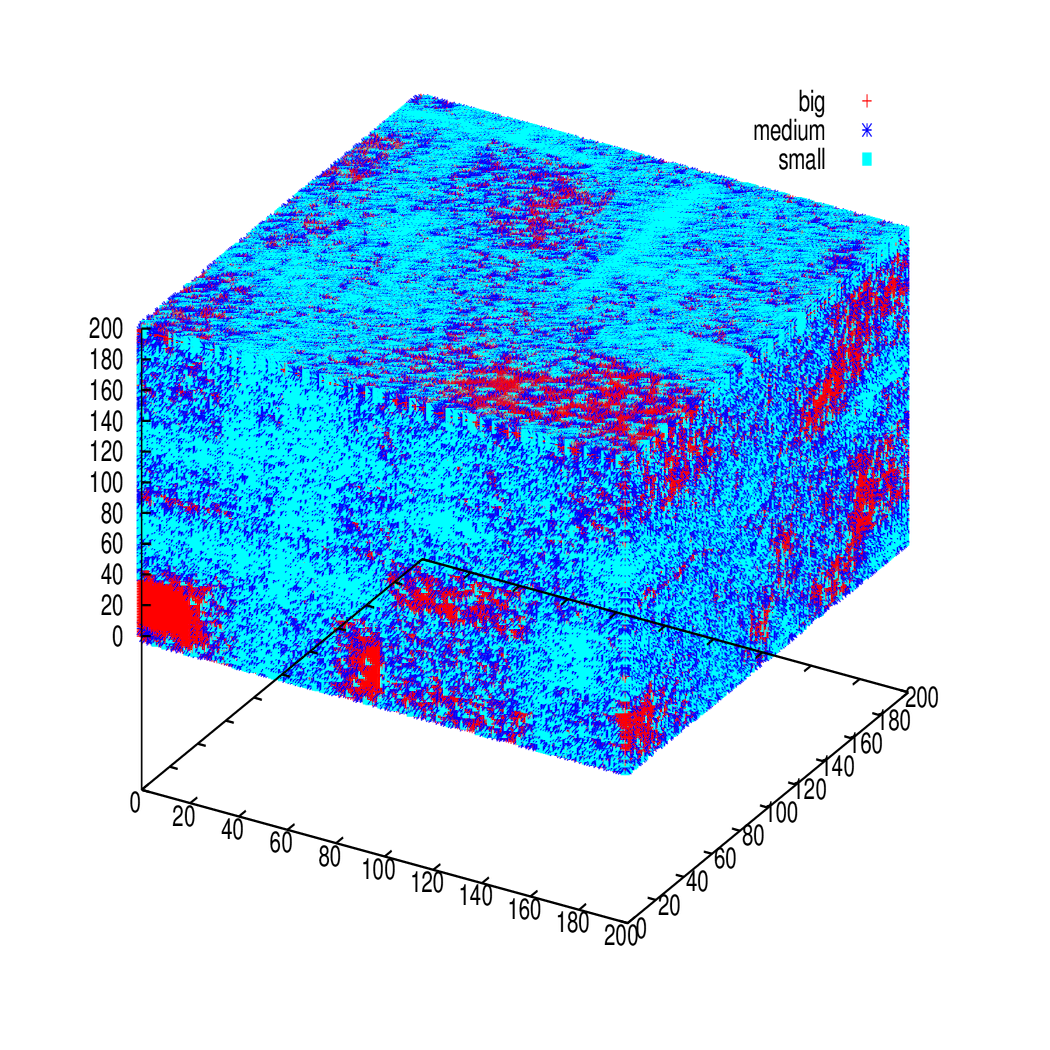
\includegraphics[width=1.5in]{img/red5.png}
%\label{fig:red5}}
%& \subfloat[$ $]{
%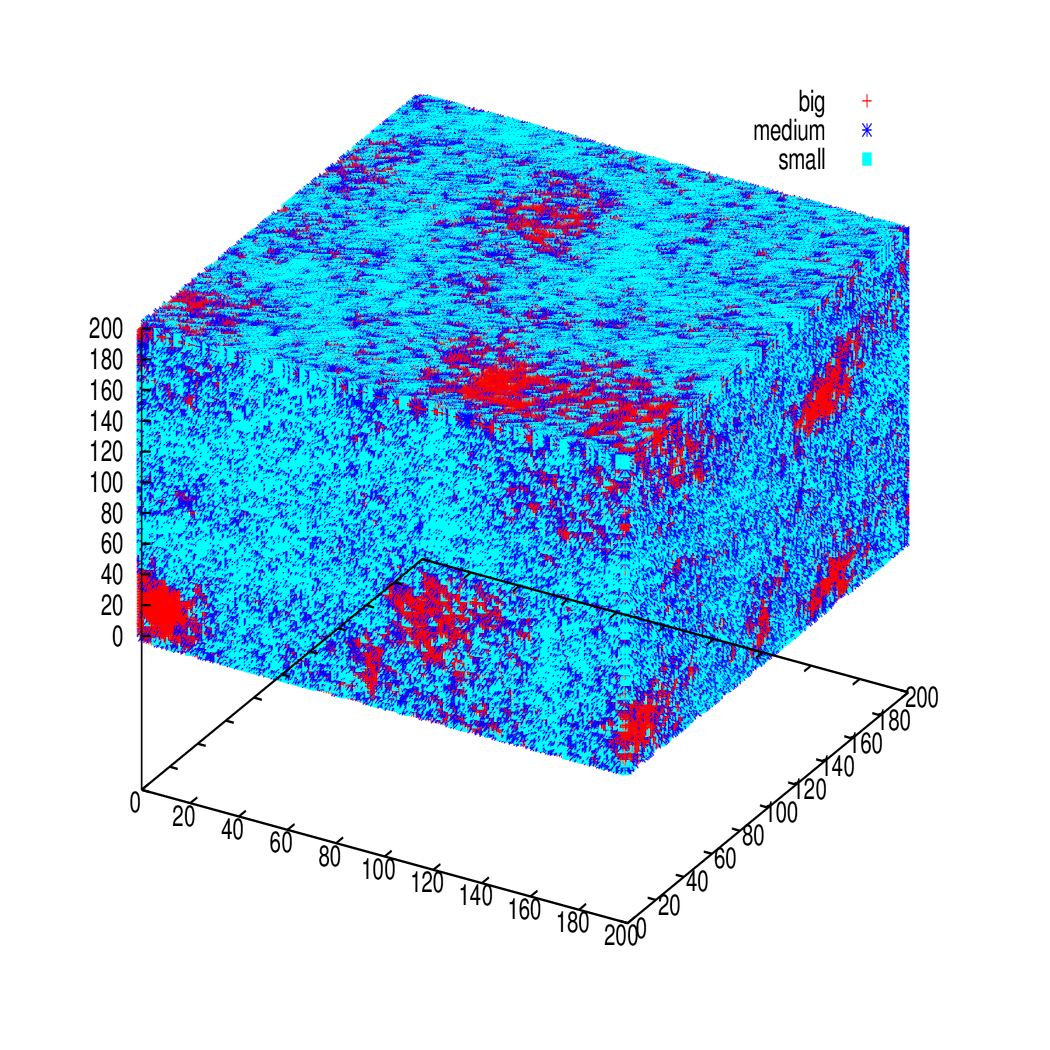
\includegraphics[width=1.5in]{img/red6.png}
%\label{fig:red6}}
%\end{tabular}
%\caption{Pore networks with additional application of $MCs$, obtained from the Parallel BSGR with $L=200$ and $\Omega=0.15$, (a) using 2 threads and (b) using 8 threads}
%\label{fig:redes3}
%\end{figure}

\begin{figure}[t]
\centering
\begin{tabular}{cc}
\subfloat[$ $]{
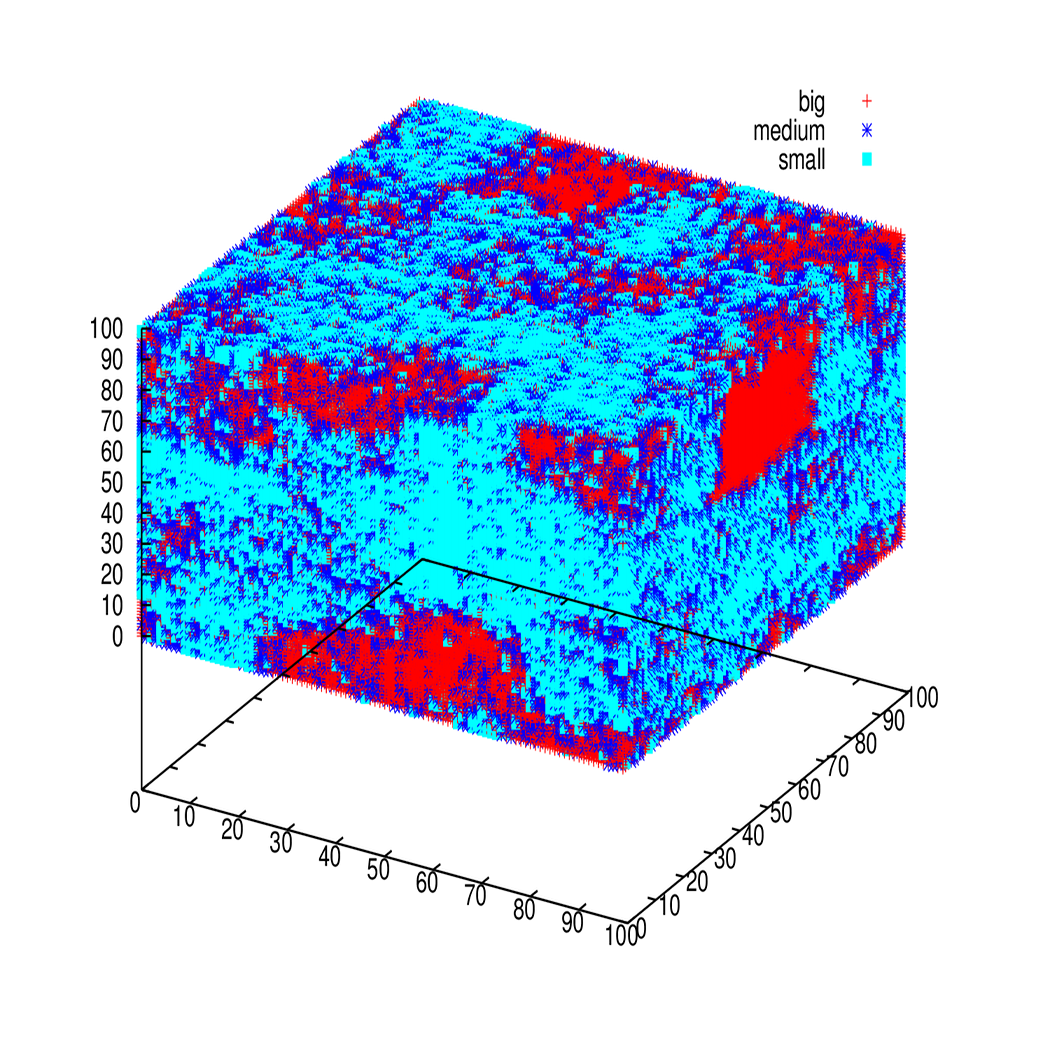
\includegraphics[width=2.3in]{img/red7.png}
\label{fig:red5}}
& \subfloat[$ $]{
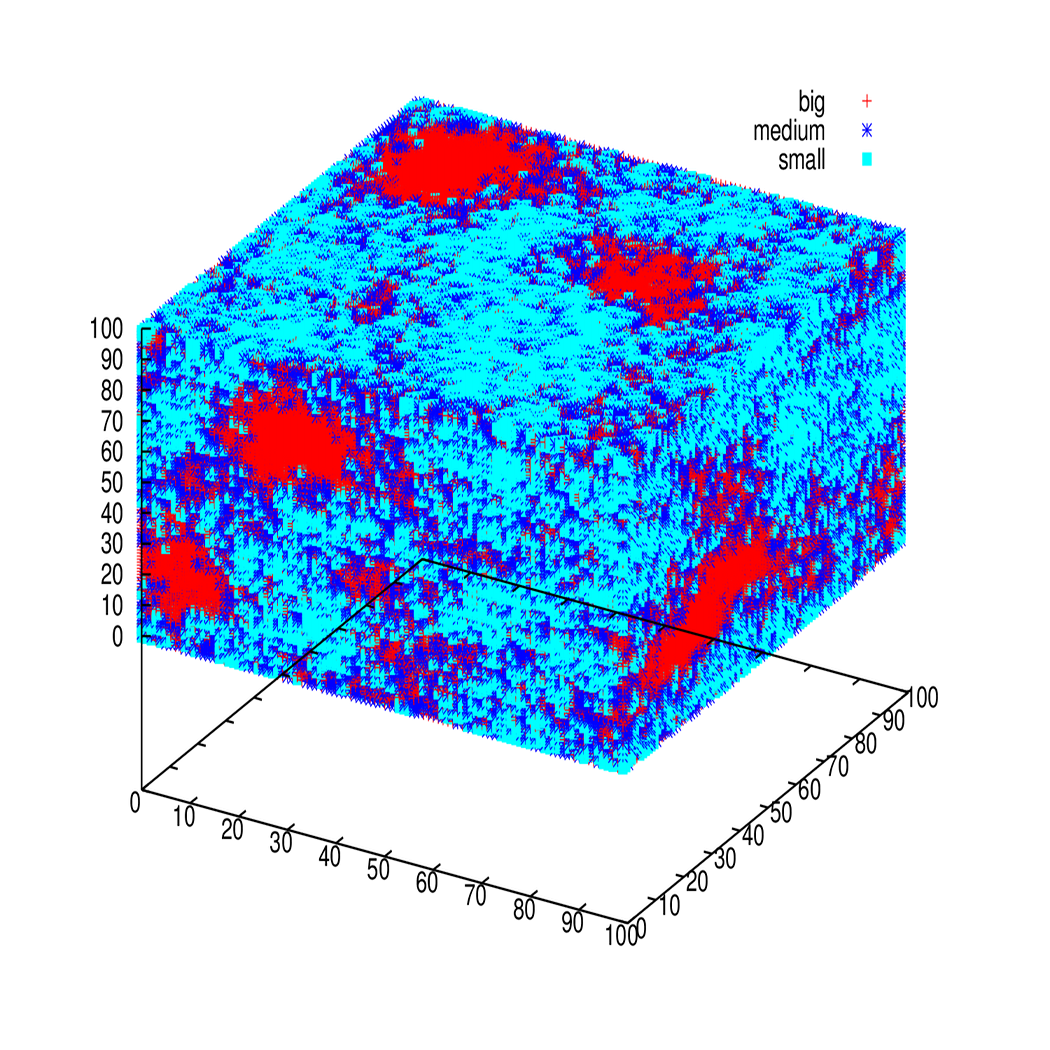
\includegraphics[width=2.3in]{img/red8.png}
\label{fig:red6}}
\end{tabular}
\caption{Redes porosas después de aplicar 2,000 $MCs$ adicionales, con L Pore networks after the application of 2000 additional $MCs$, con $L=100$ y $\Omega=0.15$, obtenidas con (a) BSGR  and (b) BSGR Paralelo utilizando 8 hilos}
\label{fig:redes3}
\end{figure}
